\documentclass[fleqn]{ctexart}
\usepackage{graphicx}
\usepackage{xcolor}
% 数学支持（提供 \mathbb、\dfrac 等）
\usepackage{amsmath,amssymb}
% 页面与版式设置：更小的页边距与顶部空白
\usepackage[a4paper,top=15mm,bottom=20mm,left=12mm,right=12mm]{geometry}
% 自动换行与字偶距优化
\usepackage{microtype}
\microtypesetup{tracking=true,protrusion=true,final}
% 在需要时放宽断行以避免溢出（数值可按需调整）
\setlength{\emergencystretch}{2em}
% 列表控制，便于让(1)后直接跟内容
\usepackage{enumitem}
% verbatim 环境支持（用于直接粘贴源码与输出）
\usepackage{verbatim}
\usepackage{fancyvrb}
\usepackage{float}
\usepackage{fvextra}
\RecustomVerbatimEnvironment{verbatim}{Verbatim}{
	frame=single,
	framesep=2mm,
	breaklines=true,
	breakanywhere=true
}
% 使章节标题左对齐（同时保留 ctex 默认样式）
\ctexset{section={format+=\raggedright}}
%1.3倍行距
\renewcommand{\baselinestretch}{1.3}
% 数学左对齐缩进为0
\setlength{\mathindent}{0pt}
% 增大矩阵的行距
\renewcommand{\arraystretch}{1.3}
\pagestyle{empty}
\begin{document}
\section*{题目1}

\subsection*{(1) 磁盘块空闲状态管理}
\textbf{思路}：计算内存空间包含的比特数，与磁盘块数作比较。
$$ 2\text{KB} = 2 \times 1024 \times 8 \text{ bits} = 16384 \text{ bits} $$
内存的位数量（16384）正好对应 16384 个磁盘块。因此，可以采用\textbf{位示图法（Bitmap）}，使用 1个 bit 来记录 1个磁盘块的空闲状态（0代表空闲，1代表已分配）。

\subsection*{(2) 读取时间计算}
\textbf{思路}：总读取时间 $T = T_{seek} (\text{寻道}) + T_{rot} (\text{旋转}) + T_{trans} (\text{传输})$。\\
\textbf{公式与计算}：
\begin{itemize}
    \item \textbf{寻道时间 $T_{seek}$}：采用 C-SCAN ，初始向大磁道号方向移动，访问序列为 $100 \rightarrow 120 \rightarrow 30 \rightarrow 50 \rightarrow 90$。
    $$ T_{seek} = (|120-100| + |120-30| + |50-30| + |90-50|) \times 1\text{ms} = (20 + 90 + 20 + 40) \text{ms} = 170\text{ms} $$
    \item \textbf{旋转延迟 $T_{rot}$}：单圈时间 $T_c = \frac{60}{6000}\text{s} = 10\text{ms}$，平均每次等待半圈 $\frac{1}{2} T_c = 5\text{ms}$。
    $$ T_{rot} = 4 \times 5\text{ms} = 20\text{ms} $$
    \item \textbf{传输时间 $T_{trans}$}：每磁道 100 扇区，单扇区读取时间为 $\frac{10\text{ms}}{100} = 0.1\text{ms}$。
    $$ T_{trans} = 4 \times 0.1\text{ms} = 0.4\text{ms} $$
    \item \textbf{总时间 $T$}：
    $$ T = T_{seek} + T_{rot} + T_{trans} = 170 + 20 + 0.4 = 190.4\text{ms} $$
\end{itemize}

\subsection*{(3) Flash设备的替代方法}
SSD 不存在机械硬盘的磁头寻道时间和盘片旋转延迟，因此使用\textbf{FCFS}即可。由于存取不同位置的时间相同，省去磁道排序计算开销可以降低延迟。

\section*{题目2}
%插入一张图片
\begin{figure}[H]
	\centering
	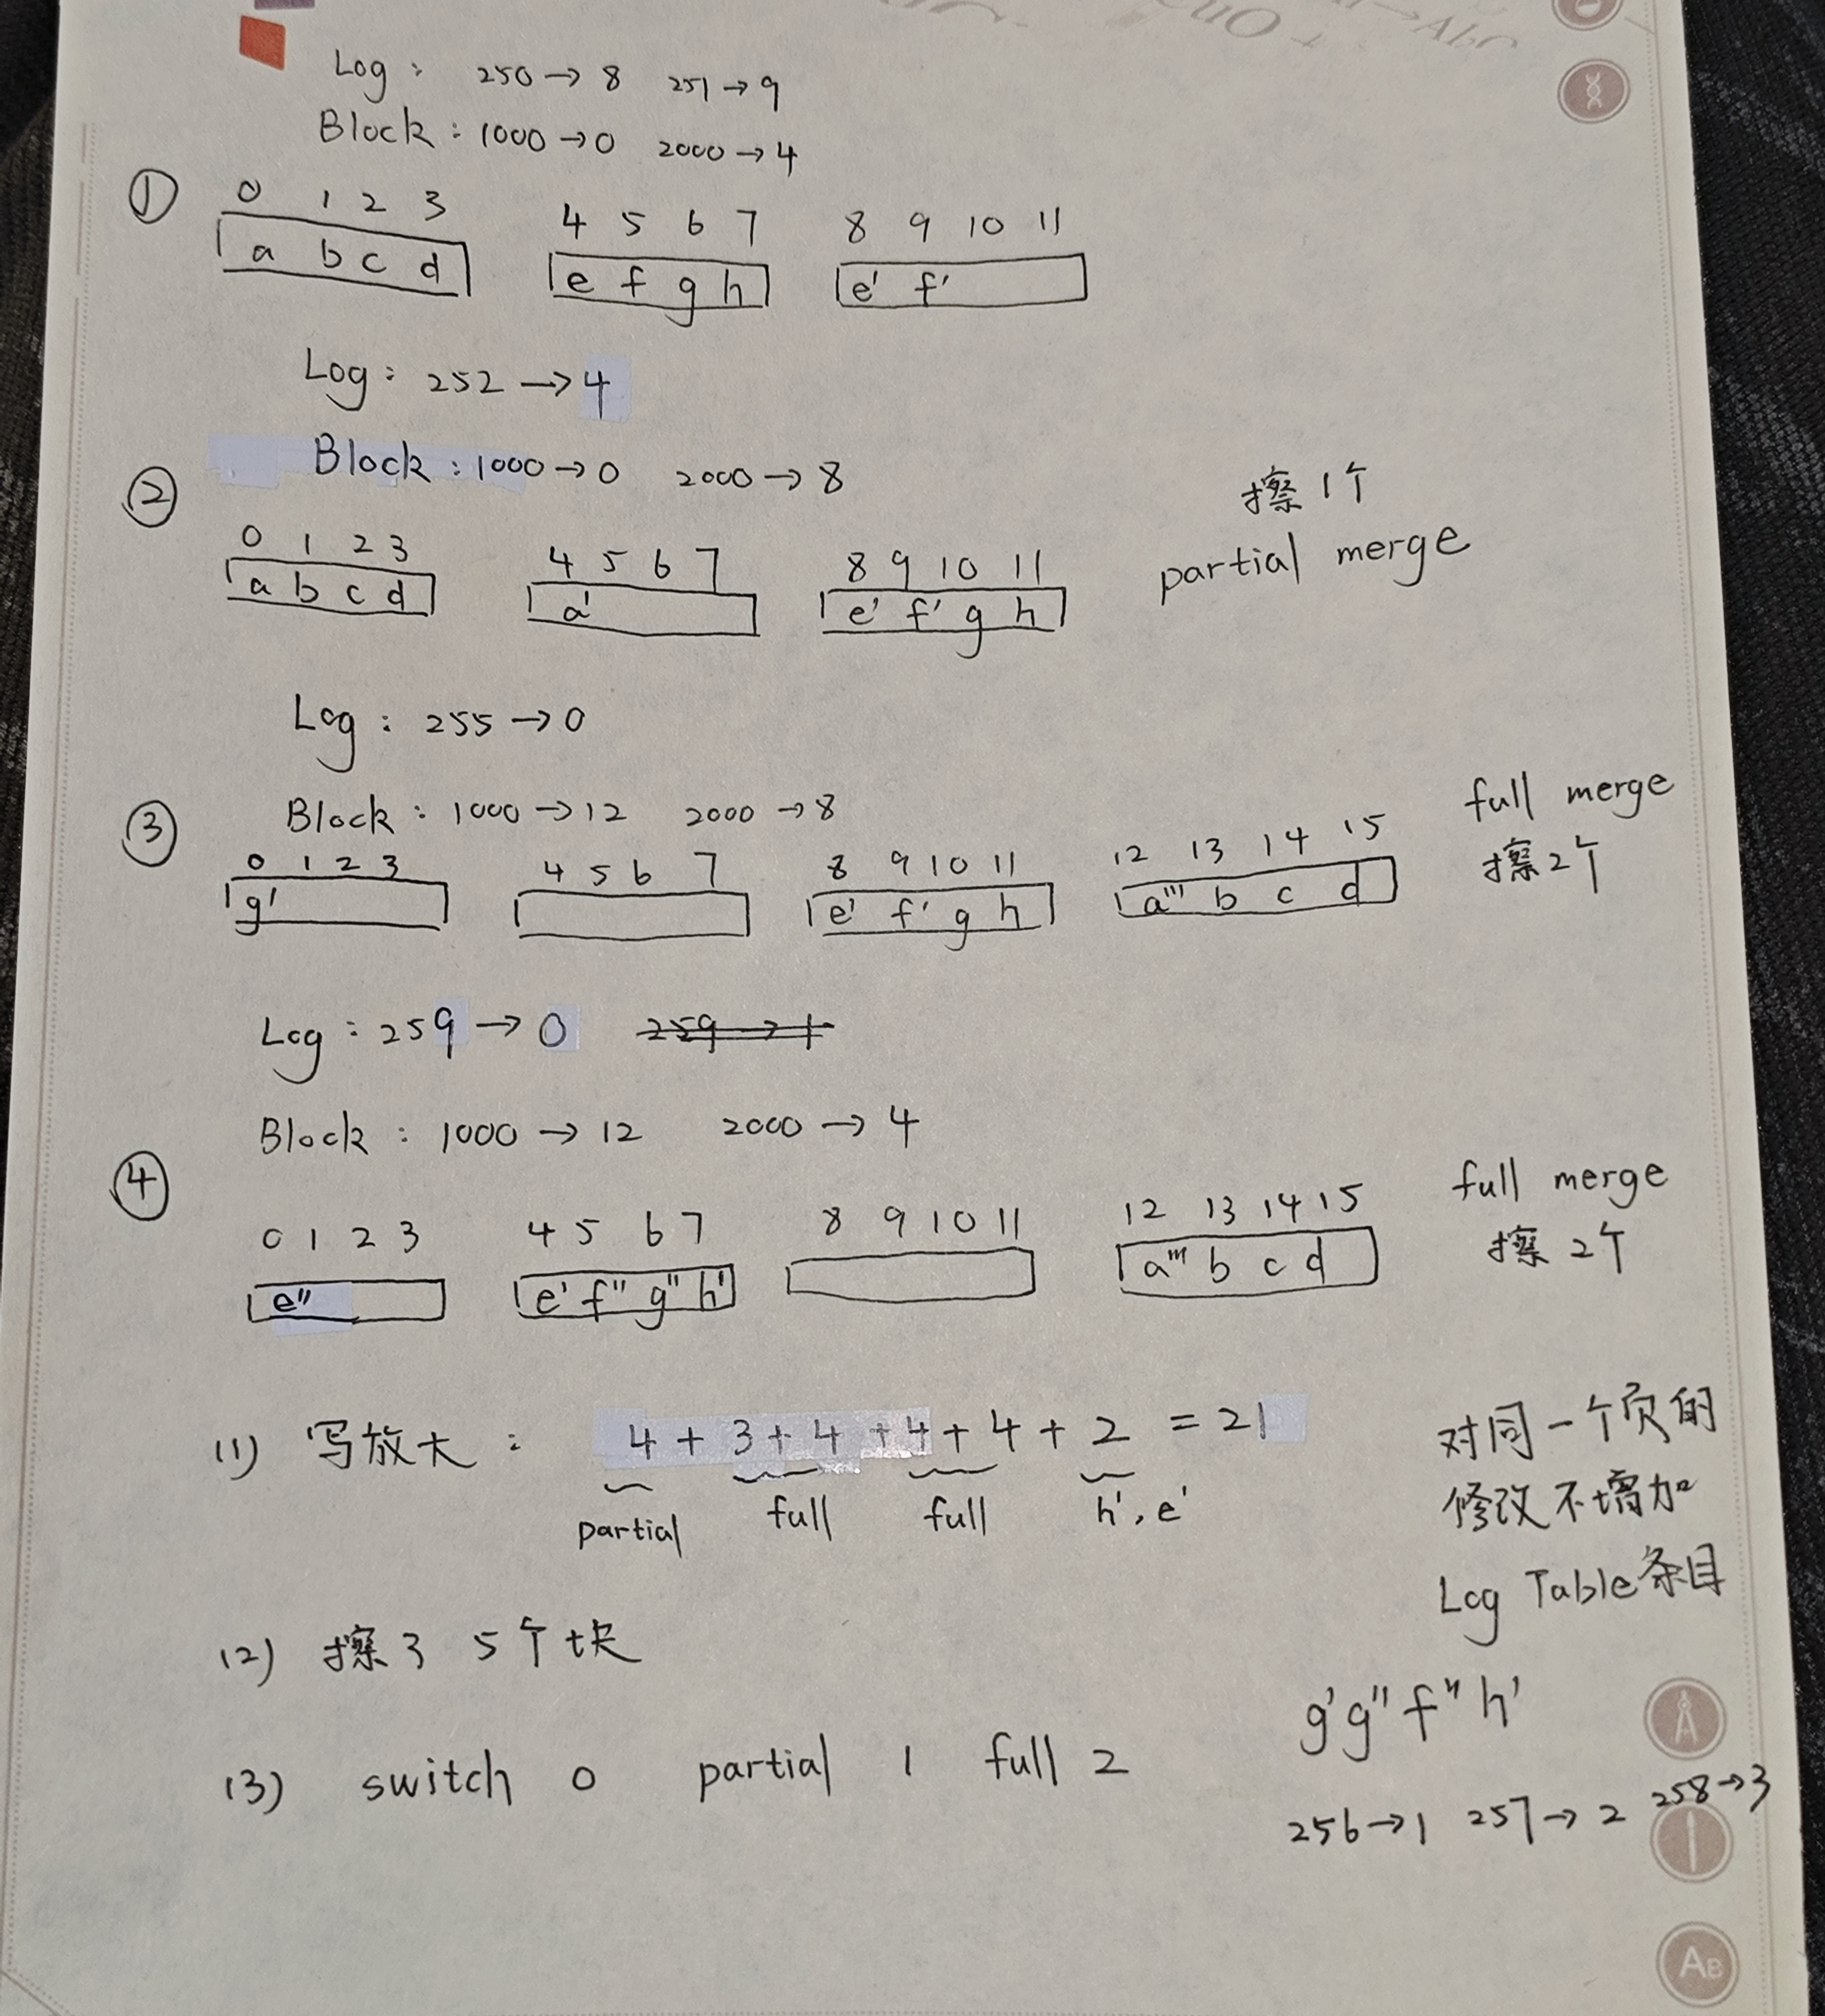
\includegraphics[width=0.8\textwidth]{image.jpg}
\end{figure}

\section*{题目3}
$fd1=3,fd2=4$，因为012已经在程序启动时被占用，分别对应标准输入、输出、错误。

父进程读一个字符，子进程读两个字符。由于共享文件的特性，父子进程的描述符完全一致，且指向同一个文件表项，因此当前文件位置也是共享的。

情况1：
\begin{verbatim}
fd2=4,child:c=b
fd2=4,c=a
fd2=4,c=r
\end{verbatim}

情况2：
\begin{verbatim}
fd2=4,c=b
fd2=4,child:c=a
fd2=4,c=r
\end{verbatim}
\end{document}